% ============================================================================
%  COMPILE WITH XeLaTeX  (twice, so the point total resolves)
%  Overleaf: Menu -> Compiler -> XeLaTeX
%  Requires: bnhandout.sty and fonts/Kalpurush.ttf in the project
% ============================================================================
\documentclass[11pt]{article}
\usepackage{bnhandout}          % add [nosol] for a student edition

\hauthor[https://sites.google.com/view/jugantordey/home]{Jugantor Dey}
\hseries{\textit{Mathematics for the Physics Olympiad}}

\begin{document}

\handouttitle{Chapter 11 : Euclidean Geometry II (Solid Geometry)}

\noindent
শুরু করার আগে ৫ নম্বর অধ্যায় থেকে ত্রিভুজের সর্বসমতা, সদৃশতা ও Pythagoras-এর
উপপাদ্য, এবং ৭ নম্বর অধ্যায় থেকে $\sin$, $\cos$, $\tan$-এর সংজ্ঞা একবার
ঝালিয়ে নাও। এই অধ্যায়ে নতুন কোনো ভারী যন্ত্রপাতি লাগবে না; যা লাগবে তা হলো
ওই দুটির উপর দাঁড়িয়ে তিন মাত্রায় ভাবতে শেখা।

সমতলের জ্যামিতি থেকে ঘন জ্যামিতিতে আসাটা কেবল একটা মাত্রা যোগ করা নয়। কাগজে যা
আঁকা যায় তা দুই মাত্রার, তাই তিন মাত্রার বস্তুকে আমরা সবসময় একটা ছায়া বা প্রক্ষেপ
হিসেবেই দেখি; আসল কাজটা হয় মাথার ভেতরে। এই কারণেই এই অধ্যায়ে সূত্র মুখস্থ
করার চেয়ে বেশি জোর দেওয়া হয়েছে দুটি অভ্যাসে: ঘনবস্তুকে কেটে তার প্রস্থচ্ছেদ
(cross-section) দেখা, আর তাকে খুলে সমতলে বিছিয়ে (net) ফেলা। এই দুটি অভ্যাস
থাকলে বেশিরভাগ সূত্র নিজে থেকেই বেরিয়ে আসে।

শেষ অনুচ্ছেদের বিষয় solid angle, যা কোণের ত্রিমাত্রিক রূপ। এটি এখানে কেবল
পরিচয় করিয়ে দেওয়া হচ্ছে; ২১ নম্বর অধ্যায়ে Gauss-এর সূত্র বুঝতে গিয়ে এটিই
সবচেয়ে বেশি কাজে লাগবে। এই অধ্যায়ে মোট \totalpoints\ পয়েন্ট আছে।

\section{তল ও ঘনবস্তু}

সমতলের জ্যামিতিতে দুটি সরলরেখা হয় ছেদ করে, নয়তো সমান্তরাল। তিন মাত্রায় তৃতীয়
একটি সম্ভাবনা আছে: দুটি রেখা ছেদও করে না, সমান্তরালও নয়, কেবল ভিন্ন দুটি সমতলে
পড়ে থাকে। এদের বলে বিষমতলীয় বা skew রেখা। ঘরের মেঝের এক প্রান্তের রেখা আর
বিপরীত দেয়ালের ছাদ-সংলগ্ন রেখা এমনই দুটি রেখা। এই একটিমাত্র উদাহরণই বলে দেয় যে
সমতলের ইন্টুইশন এখানে হুবহু খাটবে না।

\begin{idea}[সমতল]
তিনটি অসমরেখ (non-collinear) বিন্দু ঠিক একটি সমতল নির্ধারণ করে। এর কয়েকটি
সরাসরি ফল:
\begin{enumerate}
  \item দুটি ভিন্ন সমতল হয় সমান্তরাল, নয়তো একটি সরলরেখায় ছেদ করে।
  \item একটি সরলরেখা ও একটি সমতলের সম্পর্ক তিন রকম: রেখাটি সমতলে থাকে, সমতলের
        সমান্তরাল হয়, অথবা ঠিক একটি বিন্দুতে সমতলকে ছেদ করে।
  \item দুটি ছেদী সরলরেখা একটিমাত্র সমতল নির্ধারণ করে; একটি রেখা ও তার বাইরের
        একটি বিন্দুও তাই।
\end{enumerate}
\end{idea}

কেন তিনটি বিন্দু লাগে, দুটি নয়? দুটি বিন্দু দিয়ে অসংখ্য সমতল যেতে পারে, ঠিক
যেমন একটি খোলা দরজার কব্জার রেখাটি ধরে দরজা যেকোনো কোণে থাকতে পারে। তৃতীয়
বিন্দুটি সেই ঘূর্ণনটুকু আটকে দেয়। একই কারণে তিন পায়ের টুল কখনো নড়ে না, চার
পায়ের চেয়ারের একটি পা প্রায়ই মাটি ছোঁয় না।

\begin{idea}[লম্বতা ও কোণ]
একটি সরলরেখাকে বলা হয় কোনো সমতলের উপর লম্ব, যদি সে ওই সমতলের ভেতরের প্রতিটি
রেখার উপর লম্ব হয়। ব্যবহারিক পরীক্ষা: রেখাটি যদি সমতলের ভেতরের \emph{দুটি ছেদী}
রেখার উপর লম্ব হয়, তবে সে গোটা সমতলের উপরেই লম্ব।

এর উপর দাঁড়িয়ে দুটি সংজ্ঞা:
\begin{enumerate}
  \item একটি রেখা ও একটি সমতলের মধ্যেকার কোণ হলো রেখাটি এবং সমতলে তার প্রক্ষেপের
        মধ্যেকার কোণ।
  \item দুটি সমতলের মধ্যেকার কোণ, অর্থাৎ dihedral angle, মাপা হয় এভাবে: ছেদরেখার
        উপর একটি বিন্দু নাও, তারপর দুই সমতলে ছেদরেখার উপর লম্ব দুটি রশ্মি টানো;
        ওই দুই রশ্মির মধ্যেকার কোণই dihedral angle।
\end{enumerate}
\end{idea}

উপরের ``দুটি ছেদী রেখা'' পরীক্ষাটি আমরা এখানে প্রমাণ করছি না, ধরে নিচ্ছি। প্রমাণটি
কঠিন নয়, কিন্তু তাতে যে সরঞ্জাম লাগে তা ৫ নম্বর অধ্যায়ে আসেনি; আর এই
অধ্যায়ের লক্ষ্য প্রমাণের চেয়ে বেশি ইন্টুইশন তৈরি করা। ব্যবহারিকভাবে এটি খুবই
চেনা: মেঝেতে একটি লাঠি খাড়া করে রাখতে হলে দুই দিকে হেলে পড়া আটকালেই যথেষ্ট।

\begin{example}
একটি আয়তাকার বাক্সের বাহু $a$, $b$, $c$। এর কর্ণ (space diagonal) $d$-এর দৈর্ঘ্য
নির্ণয় করো, এবং কর্ণটি ভূমির সঙ্গে যে কোণ করে তা বের করো।
\end{example}

\begin{solbox}
\begin{center}
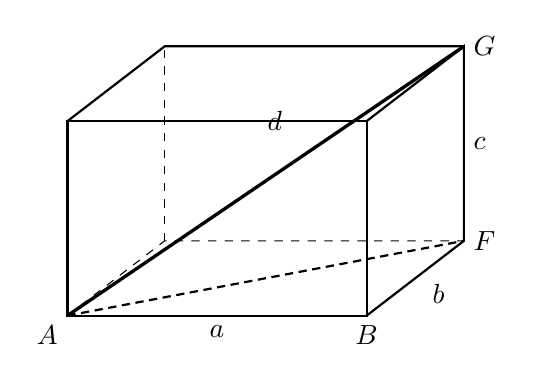
\begin{tikzpicture}[scale=0.95,>=stealth]
  \coordinate (A) at (0,0); \coordinate (B) at (4,0);
  \coordinate (C) at (4,2.6); \coordinate (D) at (0,2.6);
  \coordinate (E) at (1.3,1.0); \coordinate (F) at (5.3,1.0);
  \coordinate (G) at (5.3,3.6); \coordinate (H) at (1.3,3.6);
  \draw[thick] (A)--(B)--(C)--(D)--cycle;
  \draw[thick] (B)--(F)--(G)--(C);
  \draw[thick] (D)--(H)--(G);
  \draw[dashed] (A)--(E)--(F);
  \draw[dashed] (E)--(H);
  \draw[very thick] (A)--(G);
  \draw[thick,dash pattern=on 3pt off 2pt] (A)--(F);
  \node[below left] at (A) {$A$};
  \node[below] at (B) {$B$};
  \node[right] at (F) {$F$};
  \node[right] at (G) {$G$};
  \node[below] at (2,0) {$a$};
  \node[below right] at (4.75,0.55) {$b$};
  \node[right] at (5.3,2.3) {$c$};
  \node[above left] at (3.0,2.35) {$d$};
\end{tikzpicture}
\end{center}

কৌশলটি হলো একবারে তিন মাত্রায় না ভেবে দুই ধাপে দুবার Pythagoras প্রয়োগ করা।

\textbf{ধাপ ১।} ভূমির উপর কর্ণ $AF$ বিবেচনা করি। $ABF$ একটি সমকোণী ত্রিভুজ,
যার বাহু $a$ ও $b$, তাই
\[
  AF^{2} = a^{2} + b^{2} .
\]

\textbf{ধাপ ২।} এবার $AFG$ ত্রিভুজ। $FG$ খাড়া বাহু, তাই সে ভূমির উপর লম্ব;
বিশেষ করে $AF$-এর উপরেও লম্ব। সুতরাং $AFG$ও সমকোণী, এবং
\[
  d^{2} = AF^{2} + FG^{2} = a^{2} + b^{2} + c^{2} .
\]

কোণের জন্য: কর্ণ $AG$-এর ভূমিতে প্রক্ষেপ হলো $AF$, তাই কাঙ্ক্ষিত কোণ $\theta =
\angle GAF$। সমকোণী ত্রিভুজ $AFG$ থেকে
\[
  \tan \theta = \frac{c}{\sqrt{a^{2}+b^{2}}} .
\]
ঘনক (cube) হলে $a = b = c$, তাই $d = a\sqrt{3}$ এবং
$\tan\theta = 1/\sqrt{2}$, অর্থাৎ $\theta \approx 35.3^{\circ}$।
\end{solbox}

\begin{remark}
কাগজে তিন মাত্রা আঁকার তিনটি নিয়ম মনে রাখলে ছবি অনেক পরিষ্কার হয়। এক, যে ধারগুলো
বস্তুর পেছনে লুকিয়ে আছে সেগুলো ভাঙা রেখায় আঁকো। দুই, বাস্তবে যে ধারগুলো
সমান্তরাল, ছবিতেও সেগুলো সমান্তরাল রাখো। তিন, সমকোণকে ছবিতে সমকোণ দেখানোর চেষ্টা
কোরো না; প্রক্ষেপে কোণ বদলে যায়, দৈর্ঘ্যও বদলে যায়। ছবিটি হিসাব করার যন্ত্র নয়,
কোন ত্রিভুজে Pythagoras লাগাবে তা ঠিক করার মানচিত্র।
\end{remark}

\prob{2} একটি আয়তাকার বাক্সের বাহু $3$, $4$ ও $12$ একক।
\begin{enumerate}
  \item এর কর্ণের দৈর্ঘ্য নির্ণয় করো।
  \item $12$ বাহুটিকে উচ্চতা ধরলে কর্ণটি ভূমির সঙ্গে কত কোণ করে?
\end{enumerate}

\begin{sol}
\begin{enumerate}
  \item $d = \sqrt{3^{2}+4^{2}+12^{2}} = \sqrt{9+16+144} = \sqrt{169} = 13$।
  \item ভূমির কর্ণ $\sqrt{3^{2}+4^{2}} = 5$, তাই
        $\tan\theta = \dfrac{12}{5}$, অর্থাৎ $\theta \approx 67.4^{\circ}$।
        যাচাই: $5$, $12$, $13$ একটি চেনা ত্রিভুজ, তাই
        $\sin\theta = 12/13$ও বটে।
\end{enumerate}
\end{sol}

\prob{2} একটি ঘনকের একটি শীর্ষবিন্দুতে মিলিত দুটি তলের কর্ণের মধ্যেকার কোণ নির্ণয়
করো।

\begin{sol}
ঘনকের বাহু $a$ ধরি। একটি শীর্ষবিন্দু থেকে দুটি ভিন্ন তলের কর্ণ টানলে তাদের
অপর প্রান্ত দুটি ঘনকের আরও দুটি শীর্ষবিন্দু, আর ওই দুই প্রান্তকে যোগ করলে যে
রেখাংশ পাওয়া যায় সেটিও একটি তলের কর্ণ। সুতরাং তিনটি বাহুই $a\sqrt{2}$, অর্থাৎ
ত্রিভুজটি সমবাহু এবং কাঙ্ক্ষিত কোণ $60^{\circ}$।

সূত্র ছাড়াই এটি মনে রাখা যায়: ঘনকের যেকোনো শীর্ষবিন্দু থেকে তিনটি তলকর্ণ টানলে
একটি সমবাহু ত্রিভুজ তৈরি হয়।
\end{sol}

\prob{3} একটি ঘরের দৈর্ঘ্য ৬ মিটার, প্রস্থ ৪ মিটার, উচ্চতা ৩ মিটার। একটি মাকড়সা
মেঝের এক কোণে আছে এবং তাকে ঠিক বিপরীত কোণে (ছাদের) পৌঁছাতে হবে, তবে সে কেবল
দেয়াল, মেঝে ও ছাদ বেয়ে হাঁটতে পারে, শূন্যে উড়তে পারে না। সবচেয়ে ছোট পথের
দৈর্ঘ্য কত?

\begin{sol}
তলের উপর দিয়ে ছোট পথ খুঁজতে হলে তলগুলোকে খুলে সমতলে বিছিয়ে দাও; সমতলে সবচেয়ে
ছোট পথ সরলরেখা, তাই খোলা ছবিতে সরলরেখা টেনে তার দৈর্ঘ্য মাপলেই হলো। কোন কোন তল
পেরোনো হবে তার উপর তিন রকম খোলা সম্ভব, তাই তিনটিই হিসাব করতে হবে:
\[
  \sqrt{(6+4)^{2}+3^{2}} = \sqrt{109} \approx 10.44, \qquad
  \sqrt{(6+3)^{2}+4^{2}} = \sqrt{97} \approx 9.85,
\]
\[
  \sqrt{(4+3)^{2}+6^{2}} = \sqrt{85} \approx 9.22 .
\]
সবচেয়ে ছোট পথ $\sqrt{85} \approx 9.22$ মিটার।

তুলনা করার মতো: সরাসরি উড়ে গেলে লাগত $\sqrt{6^{2}+4^{2}+3^{2}} = \sqrt{61}
\approx 7.81$ মিটার। আর ``আগে মেঝে বরাবর সোজা, তারপর দেয়াল বেয়ে খাড়া উপরে''
এই স্বাভাবিক মনে হওয়া পথটির দৈর্ঘ্য $\sqrt{52} + 3 \approx 10.21$ মিটার, যা
সবচেয়ে ছোট নয়। খুলে ফেলার কৌশলটাই এখানে আসল কথা।
\end{sol}

\section{প্রিজম ও পিরামিড}

\begin{idea}[Prism]
দুটি সর্বসম ও সমান্তরাল বহুভুজ তল (base) এবং তাদের সংযোগকারী সামান্তরিক তল
নিয়ে গঠিত ঘনবস্তুকে বলে prism। পার্শ্বতলগুলো ভূমির উপর লম্ব হলে একে বলে right
prism। যেকোনো prism-এর জন্য
\[
  V = Bh ,
\]
যেখানে $B$ ভূমির ক্ষেত্রফল এবং $h$ উচ্চতা, অর্থাৎ দুই ভূমির মধ্যেকার লম্ব দূরত্ব।
\end{idea}

কেন এটি সত্য, তার ছবিটা সহজ: prism-কে ভাবো একই আকারের অসংখ্য পাতলা কাগজের
স্তূপ হিসেবে। প্রতিটি পাতার ক্ষেত্রফল $B$, আর মোট উচ্চতা $h$। এখন স্তূপটাকে
একদিকে হেলিয়ে দিলে (অর্থাৎ oblique prism বানালে) পাতার সংখ্যা বা তাদের ক্ষেত্রফল
কিছুই বদলায় না, তাই আয়তনও বদলায় না।

এই যুক্তিটুকু আমরা এখানে একটি নীতি হিসেবে ধরে নেব: \emph{দুটি ঘনবস্তুর ভূমি একই
সমতলে থাকলে এবং প্রতিটি উচ্চতায় তাদের প্রস্থচ্ছেদের ক্ষেত্রফল সমান হলে, তাদের
আয়তনও সমান।} এটি প্রমাণ করা হচ্ছে না; ১৭ নম্বর অধ্যায়ে integration হাতে এলে
এটি এক লাইনে বেরিয়ে আসবে, কারণ আয়তন তখন হবে প্রস্থচ্ছেদের ক্ষেত্রফলের যোগফল।
আপাতত কাগজের স্তূপের ছবিটাই যথেষ্ট।

\begin{idea}[Pyramid]
একটি বহুভুজ ভূমি এবং ভূমির বাইরের একটি শীর্ষবিন্দু (apex) নিয়ে গঠিত ঘনবস্তুকে
বলে pyramid। এর আয়তন
\[
  V = \frac{1}{3} Bh .
\]
ভূমি সুষম বহুভুজ এবং apex ভূমির কেন্দ্রের ঠিক উপরে থাকলে পার্শ্বতলের ক্ষেত্রফল
\[
  A_{\mathrm{lat}} = \frac{1}{2}\, p \, l ,
\]
যেখানে $p$ ভূমির পরিসীমা এবং $l$ হলো slant height, অর্থাৎ apex থেকে ভূমির কোনো
বাহুর মধ্যবিন্দু পর্যন্ত দূরত্ব। এই অধ্যায়ে $A_{\mathrm{lat}}$ মানে
পার্শ্বতলের ক্ষেত্রফল এবং $A_{\mathrm{tot}}$ মানে মোট পৃষ্ঠতল।
\end{idea}

$\tfrac{1}{3}$ ভগ্নাংশটি কোথা থেকে এল, সেটা একটা ঘনক কেটে দেখা যায়।

\begin{center}
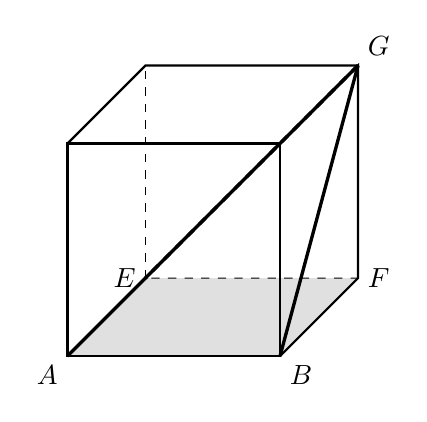
\begin{tikzpicture}[scale=0.9,>=stealth]
  \coordinate (A) at (0,0); \coordinate (B) at (3,0);
  \coordinate (C) at (3,3); \coordinate (D) at (0,3);
  \coordinate (E) at (1.1,1.1); \coordinate (F) at (4.1,1.1);
  \coordinate (G) at (4.1,4.1); \coordinate (H) at (1.1,4.1);
  \fill[black!12] (A)--(B)--(F)--(E)--cycle;
  \draw[thick] (A)--(B)--(C)--(D)--cycle;
  \draw[thick] (B)--(F)--(G)--(C);
  \draw[thick] (D)--(H)--(G);
  \draw[dashed] (A)--(E)--(F);
  \draw[dashed] (E)--(H);
  \draw[very thick] (G)--(A); \draw[very thick] (G)--(B);
  \draw[very thick,dashed] (G)--(E);
  \node[below left] at (A) {$A$};
  \node[below right] at (B) {$B$};
  \node[right] at (F) {$F$};
  \node[above right] at (G) {$G$};
  \node[left] at (E) {$E$};
\end{tikzpicture}
\end{center}

$a$ বাহুর একটি ঘনক নাও এবং একটি শীর্ষবিন্দু $G$ বেছে নাও। $G$ যে তিনটি তলে নেই,
সেই তিনটিকে ভূমি ধরে $G$-কে apex বানালে তিনটি pyramid পাওয়া যায়। ছবিতে তার একটি
দেখানো হয়েছে: ভূমি $ABFE$ এবং apex $G$। এই তিনটি pyramid ঘনকটিকে ঠিক ঠিক ভরে
ফেলে, একটুও ফাঁক থাকে না, একটুও ওভারল্যাপ হয় না; আর তিনটি একে অপরের সর্বসম, কারণ
ঘনকটিকে ঘুরিয়ে একটিকে অন্যটির উপর বসিয়ে দেওয়া যায়। সুতরাং প্রতিটির আয়তন
$a^{3}/3$। এদিকে প্রতিটির ভূমির ক্ষেত্রফল $a^{2}$ এবং উচ্চতা $a$ (যেমন ছবির
pyramid-টির উচ্চতা হলো $GF$)। তাই
\[
  V = \frac{a^{3}}{3} = \frac{1}{3} \cdot a^{2} \cdot a = \frac{1}{3} Bh .
\]

এটি কেবল একটি বিশেষ pyramid-এর হিসাব। সাধারণ pyramid-এর জন্য একই $\tfrac{1}{3}$
আসে উপরের প্রস্থচ্ছেদের নীতি থেকে: apex থেকে $y$ দূরত্বে যেকোনো pyramid-এর
প্রস্থচ্ছেদ ভূমির সদৃশ, আর সদৃশ আকৃতির ক্ষেত্রফল দৈর্ঘ্যের বর্গের সমানুপাতিক
(এই কথাটা চার নম্বর অনুচ্ছেদে বিস্তারিত আসছে)। তাই একই উচ্চতা ও একই ভূমি-ক্ষেত্রফলের
দুটি pyramid-এর প্রতিটি উচ্চতায় প্রস্থচ্ছেদ সমান, সুতরাং আয়তনও সমান। ভূমি
বর্গাকার হোক বা ত্রিভুজাকার বা বৃত্তাকার, $\tfrac{1}{3}$ বদলায় না।

\begin{example}
একটি সুষম চতুর্ভুজাকার pyramid-এর ভূমির বাহু ১০ একক এবং উচ্চতা ১২ একক। এর slant
height, পার্শ্বতলের ক্ষেত্রফল, মোট পৃষ্ঠতল ও আয়তন নির্ণয় করো।
\end{example}

\begin{solbox}
Apex ভূমির কেন্দ্রের উপরে। কেন্দ্র থেকে ভূমির একটি বাহুর মধ্যবিন্দু পর্যন্ত দূরত্ব
বাহুর অর্ধেক, অর্থাৎ $5$। তাই slant height
\[
  l = \sqrt{12^{2} + 5^{2}} = \sqrt{169} = 13 .
\]
পার্শ্বতল চারটি সর্বসম ত্রিভুজ, প্রতিটির ভূমি $10$ ও উচ্চতা $l = 13$:
\[
  A_{\mathrm{lat}} = \frac{1}{2} \times 40 \times 13 = 260 .
\]
মোট পৃষ্ঠতল $= 260 + 10^{2} = 360$ বর্গ একক। আয়তন
\[
  V = \frac{1}{3} \times 100 \times 12 = 400 ,
\]
অর্থাৎ ৪০০ ঘন একক।
খেয়াল করো, slant height আর উচ্চতা এক জিনিস নয়। এই দুটি গুলিয়ে ফেলা এই
অনুচ্ছেদের সবচেয়ে সাধারণ ভুল; ছবিতে সমকোণী ত্রিভুজটি এঁকে ফেললে আর ভুল হয় না।
\end{solbox}

\prob{2} একটি সুষম চতুর্ভুজাকার pyramid-এর ভূমির বাহু ১৬ একক এবং উচ্চতা ৬ একক।
এর slant height, মোট পৃষ্ঠতল ও আয়তন নির্ণয় করো।

\begin{sol}
ভূমির কেন্দ্র থেকে বাহুর মধ্যবিন্দুর দূরত্ব $8$, তাই
$l = \sqrt{6^{2}+8^{2}} = 10$।

পার্শ্বতল $= \tfrac{1}{2} \times (4 \times 16) \times 10 = 320$;
মোট পৃষ্ঠতল $= 320 + 16^{2} = 576$ বর্গ একক।

আয়তন $= \tfrac{1}{3} \times 256 \times 6 = 512$ ঘন একক।
\end{sol}

\prob{2} একটি right prism-এর ভূমি সমবাহু ত্রিভুজ, যার বাহু ৬ একক, এবং prism-এর
দৈর্ঘ্য ১০ একক। এর আয়তন ও মোট পৃষ্ঠতল নির্ণয় করো।

\begin{sol}
সমবাহু ত্রিভুজের ক্ষেত্রফল $\dfrac{\sqrt{3}}{4} \times 6^{2} = 9\sqrt{3}$।
সুতরাং
\[
  V = 9\sqrt{3} \times 10 = 90\sqrt{3} \approx 155.9 ,
\]
অর্থাৎ প্রায় ১৫৫.৯ ঘন একক।
পার্শ্বতল তিনটি আয়তক্ষেত্র, প্রতিটি $6 \times 10$, মোট $180$। দুই ভূমি মিলে
$18\sqrt{3}$। মোট পৃষ্ঠতল $= 180 + 18\sqrt{3} \approx 211.2$ বর্গ একক।
\end{sol}

\prob{3} একটি সুষম চতুস্তলক (regular tetrahedron), অর্থাৎ যার চারটি তলই সমবাহু
ত্রিভুজ, তার বাহু $a$। এর উচ্চতা ও আয়তন $a$-এর মাধ্যমে প্রকাশ করো।

\begin{sol}
Apex ভূমির কেন্দ্রের ঠিক উপরে, কারণ চারটি বাহুই সমান। সমবাহু ত্রিভুজের কেন্দ্র
থেকে তার একটি শীর্ষবিন্দুর দূরত্ব হলো পরিব্যাসার্ধ $R = \dfrac{a}{\sqrt{3}}$।

Apex, কেন্দ্র এবং একটি ভূমি-শীর্ষবিন্দু নিয়ে যে সমকোণী ত্রিভুজ হয়, তার অতিভুজ
$a$ এবং একটি বাহু $R$, তাই উচ্চতা
\[
  h = \sqrt{a^{2} - \frac{a^{2}}{3}} = a\sqrt{\frac{2}{3}} = \frac{a\sqrt{6}}{3} .
\]
ভূমির ক্ষেত্রফল $\dfrac{\sqrt{3}}{4}a^{2}$, সুতরাং
\[
  V = \frac{1}{3} \cdot \frac{\sqrt{3}}{4}a^{2} \cdot \frac{a\sqrt{6}}{3}
    = \frac{\sqrt{18}}{36} a^{3} = \frac{a^{3}\sqrt{2}}{12} .
\]
মোটামুটি যাচাই: $\sqrt{2}/12 \approx 0.118$, অর্থাৎ চতুস্তলকটি $a$ বাহুর ঘনকের
প্রায় বারো ভাগের এক ভাগ জায়গা নেয়, যা ছবির সঙ্গে মানানসই।
\end{sol}

\section{সিলিন্ডার, কোণক, গোলক}

\begin{idea}[Cylinder]
Cylinder হলো বৃত্তাকার ভূমির prism। ভূমির ব্যাসার্ধ $r$ ও উচ্চতা $h$ হলে
\[
  V = \pi r^{2} h, \qquad
  A_{\mathrm{lat}} = 2\pi r h, \qquad
  A_{\mathrm{tot}} = 2\pi r^{2} + 2\pi r h .
\]
\end{idea}

আয়তনের সূত্রটি prism-এর সূত্রেরই বিশেষ রূপ। পার্শ্বতলের সূত্রটি net থেকে আসে:
cylinder-এর গা বরাবর কেটে খুলে বিছিয়ে দিলে একটি আয়তক্ষেত্র পাওয়া যায়, যার
উচ্চতা $h$ এবং প্রস্থ ভূমির পরিধি $2\pi r$।

\begin{idea}[Cone]
Cone হলো বৃত্তাকার ভূমির pyramid। ব্যাসার্ধ $r$, উচ্চতা $h$ এবং slant height
$l = \sqrt{r^{2}+h^{2}}$ হলে
\[
  V = \frac{1}{3}\pi r^{2} h, \qquad
  A_{\mathrm{lat}} = \pi r l, \qquad
  A_{\mathrm{tot}} = \pi r^{2} + \pi r l .
\]
\end{idea}

\begin{center}
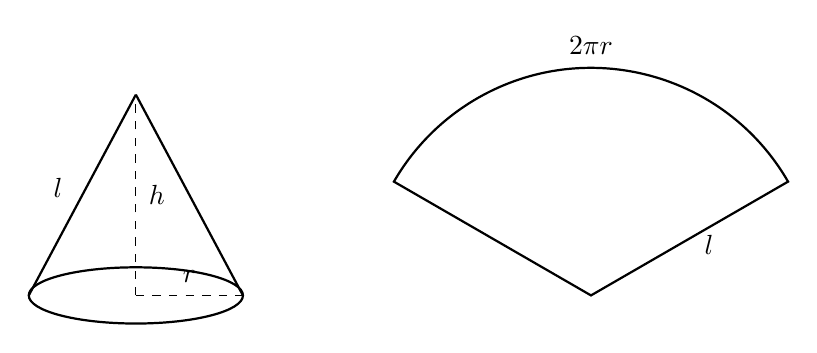
\begin{tikzpicture}[scale=0.85,>=stealth]
 \begin{scope}
  \draw[thick] (0,3) -- (-1.6,0);
  \draw[thick] (0,3) -- (1.6,0);
  \draw[thick] (0,0) ellipse (1.6 and 0.42);
  \draw[dashed] (0,0) -- (1.6,0);
  \draw[dashed] (0,0) -- (0,3);
  \node[above] at (0.8,0.04) {$r$};
  \node[right] at (0.05,1.5) {$h$};
  \node[left] at (-0.95,1.6) {$l$};
 \end{scope}
 \begin{scope}[xshift=6.8cm]
  \draw[thick] (0,0) -- (30:3.4) arc[start angle=30,end angle=150,radius=3.4] -- cycle;
  \node[below right] at (1.55,1.05) {$l$};
  \node[above] at (0,3.45) {$2\pi r$};
 \end{scope}
\end{tikzpicture}
\end{center}

পার্শ্বতলের সূত্রটি এখানে সত্যিই বের করা যায়। Cone-এর গা বরাবর একটি সরলরেখা ধরে
কেটে খুলে বিছিয়ে দাও; যা পাওয়া যায় তা একটি বৃত্তকলা (sector), যার ব্যাসার্ধ
$l$ এবং চাপের দৈর্ঘ্য ভূমির পরিধি, অর্থাৎ $2\pi r$। $l$ ব্যাসার্ধের পূর্ণ বৃত্তের
পরিধি $2\pi l$ এবং ক্ষেত্রফল $\pi l^{2}$; আমাদের sector সেই পূর্ণ বৃত্তের
$\dfrac{2\pi r}{2\pi l} = \dfrac{r}{l}$ অংশ। সুতরাং
\[
  A_{\mathrm{lat}} = \frac{r}{l} \times \pi l^{2} = \pi r l .
\]

\begin{idea}[Sphere]
$r$ ব্যাসার্ধের গোলকের জন্য
\[
  V = \frac{4}{3}\pi r^{3}, \qquad A = 4\pi r^{2} .
\]
\end{idea}

আয়তনের সূত্রটির পেছনে একটি চমৎকার ছবি আছে, যা কেবল Pythagoras ব্যবহার করে।

\begin{center}
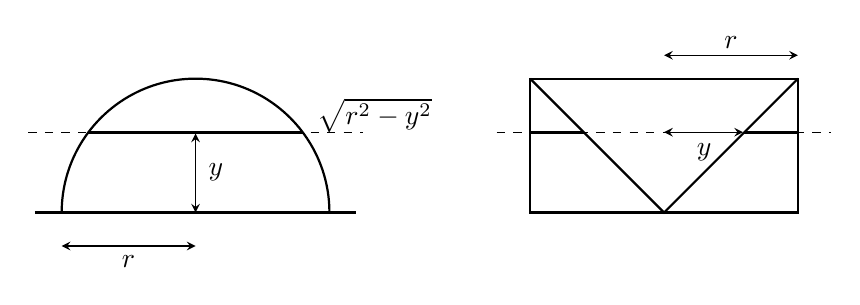
\begin{tikzpicture}[scale=0.85,>=stealth]
 \begin{scope}
  \draw[thick] (-2.4,0) -- (2.4,0);
  \draw[thick] (-2,0) arc[start angle=180,end angle=0,radius=2];
  \draw[dashed] (-2.5,1.2) -- (2.5,1.2);
  \draw[very thick] (-1.6,1.2) -- (1.6,1.2);
  \draw[<->] (0,0) -- (0,1.18);
  \node[right] at (0.05,0.6) {$y$};
  \node[right] at (1.68,1.45) {$\sqrt{r^{2}-y^{2}}$};
  \draw[<->] (-2,-0.5) -- (0,-0.5);
  \node[below] at (-1.0,-0.5) {$r$};
 \end{scope}
 \begin{scope}[xshift=7.0cm]
  \draw[thick] (-2,0) rectangle (2,2);
  \draw[thick] (-2,2) -- (0,0) -- (2,2);
  \draw[dashed] (-2.5,1.2) -- (2.5,1.2);
  \draw[very thick] (-2,1.2) -- (-1.2,1.2);
  \draw[very thick] (1.2,1.2) -- (2,1.2);
  \draw[<->] (0,1.2) -- (1.18,1.2);
  \node at (0.6,0.9) {$y$};
  \draw[<->] (0,2.35) -- (2,2.35);
  \node[above] at (1.0,2.3) {$r$};
 \end{scope}
\end{tikzpicture}
\end{center}

বাঁ দিকে $r$ ব্যাসার্ধের একটি অর্ধগোলক, সমতল দিকটি নিচে। ডান দিকে $r$ ব্যাসার্ধ ও
$r$ উচ্চতার একটি cylinder, যার ভেতর থেকে একটি cone বাদ দেওয়া হয়েছে; ওই cone-এর
শীর্ষবিন্দু নিচের কেন্দ্রে আর ভূমি cylinder-এর উপরের তল। দুটিকেই $y$ উচ্চতায়
কাটো।

অর্ধগোলকের প্রস্থচ্ছেদ একটি বৃত্ত। Pythagoras বলছে তার ব্যাসার্ধ
$\sqrt{r^{2}-y^{2}}$, তাই ক্ষেত্রফল $\pi(r^{2}-y^{2})$।

ডান দিকের প্রস্থচ্ছেদ একটি বৃত্তবলয় (ring)। বাইরের ব্যাসার্ধ $r$; ভেতরের
ব্যাসার্ধ হলো ওই উচ্চতায় cone-এর ব্যাসার্ধ, যা ঠিক $y$, কারণ cone-টি $45^{\circ}$
কোণে খোলে। তাই ক্ষেত্রফল $\pi r^{2} - \pi y^{2} = \pi (r^{2}-y^{2})$।

দুটি সমান, প্রতিটি উচ্চতায়। প্রস্থচ্ছেদের নীতি অনুযায়ী তাই আয়তনও সমান:
\[
  V_{\mathrm{hemi}} = \pi r^{2} \cdot r - \frac{1}{3}\pi r^{2} \cdot r
  = \frac{2}{3}\pi r^{3}
  \;\Longrightarrow\;
  V_{\mathrm{sph}} = \frac{4}{3}\pi r^{3} .
\]

পৃষ্ঠতলের সূত্রটিও আয়তন থেকে পাওয়া যায়। গোলকের পৃষ্ঠকে অসংখ্য ছোট ছোট টুকরোয়
ভাগ করো এবং প্রতিটি টুকরোকে কেন্দ্রের সঙ্গে জুড়ে একটি সরু pyramid বানাও। প্রতিটি
pyramid-এর উচ্চতা প্রায় $r$, আর টুকরোগুলো যত ছোট হবে ``প্রায়'' কথাটা তত ভালো
হবে। সব pyramid-এর ভূমি মিলে গোলকের পৃষ্ঠ $A$, তাই
\[
  V \approx \frac{1}{3} A r
  \;\Longrightarrow\;
  A \approx \frac{3V}{r} = \frac{3}{r} \cdot \frac{4}{3}\pi r^{3} = 4\pi r^{2} .
\]
এখানে ``প্রায়'' থেকে ``ঠিক''-এ যাওয়ার ধাপটি একটি limit, তাই এটিকে প্রমাণ না বলে
যুক্তিসঙ্গত ছবি বলাই ভালো; ১৭ নম্বর অধ্যায়ে এটি নিখুঁতভাবে করা হবে।

\begin{example}
একটি cone, একটি অর্ধগোলক ও একটি cylinder, তিনটিরই ভূমির ব্যাসার্ধ $r$ এবং উচ্চতা
$r$। এদের আয়তনের অনুপাত নির্ণয় করো।
\end{example}

\begin{solbox}
সরাসরি বসিয়ে দিই:
\[
  V_{\mathrm{cone}} = \frac{1}{3}\pi r^{3}, \qquad
  V_{\mathrm{hemi}} = \frac{2}{3}\pi r^{3}, \qquad
  V_{\mathrm{cyl}} = \pi r^{3} .
\]
সুতরাং অনুপাত $1 : 2 : 3$।

এটি নিছক কাকতালীয় নয়; উপরের ছবিতেই দেখা গেছে যে অর্ধগোলক ঠিক cylinder বিয়োগ
cone, অর্থাৎ $3 - 1 = 2$। এই একটি অনুপাত মনে রাখলে তিনটি সূত্রই মনে থাকে।
\end{solbox}

\begin{example}
একটি cone-এর ভূমির ব্যাসার্ধ ৫ একক ও slant height ১৩ একক। এর net-এর sector-টি
কত ডিগ্রি কোণের?
\end{example}

\begin{solbox}
Sector-টি $l = 13$ ব্যাসার্ধের পূর্ণ বৃত্তের $\dfrac{r}{l} = \dfrac{5}{13}$ অংশ।
সুতরাং তার কোণ
\[
  \frac{5}{13} \times 360^{\circ} \approx 138.5^{\circ} .
\]
পাশাপাশি cone-এর উচ্চতা $h = \sqrt{13^{2}-5^{2}} = 12$, তাই আয়তন
$\tfrac{1}{3}\pi \cdot 25 \cdot 12 = 100\pi$ ঘন একক।
\end{solbox}

\prob{2} একটি cone-এর ভূমির ব্যাসার্ধ ৬ একক ও উচ্চতা ৮ একক। এর slant height,
মোট পৃষ্ঠতল ও আয়তন নির্ণয় করো।

\begin{sol}
$l = \sqrt{6^{2}+8^{2}} = 10$।

মোট পৃষ্ঠতল $= \pi r^{2} + \pi r l = 36\pi + 60\pi = 96\pi$ বর্গ একক।

আয়তন $= \tfrac{1}{3}\pi \cdot 36 \cdot 8 = 96\pi$ ঘন একক।

দুটি সংখ্যা মিলে গেছে, কিন্তু এটি নিছক এই মাপগুলোর কাকতালীয় ব্যাপার; একটি
ক্ষেত্রফল আর অন্যটি আয়তন, দুটি ভিন্ন জাতের রাশি, তাই এদের সমান বলা অর্থহীন।
\end{sol}

\prob{2} একটি গোলক একটি cylinder-এর ভেতরে ঠিকঠাক এঁটে বসে আছে, অর্থাৎ দুটির
ব্যাসার্ধ সমান এবং cylinder-এর উচ্চতা গোলকের ব্যাসের সমান। দেখাও যে
\begin{enumerate}
  \item গোলকের আয়তন cylinder-এর আয়তনের ঠিক দুই-তৃতীয়াংশ;
  \item গোলকের পৃষ্ঠতল cylinder-এর পার্শ্বতলের ঠিক সমান।
\end{enumerate}

\begin{sol}
Cylinder-এর ব্যাসার্ধ $r$, উচ্চতা $2r$।
\begin{enumerate}
  \item $V_{\mathrm{cyl}} = \pi r^{2} \cdot 2r = 2\pi r^{3}$ এবং
        $V_{\mathrm{sph}} = \tfrac{4}{3}\pi r^{3}$, তাই অনুপাত
        $\dfrac{4/3}{2} = \dfrac{2}{3}$।
  \item $A_{\mathrm{cyl,lat}} = 2\pi r \cdot 2r = 4\pi r^{2}$, আর
        $A_{\mathrm{sph}} = 4\pi r^{2}$। সমান।
\end{enumerate}
\end{sol}

\prob{3} একটি cone-আকৃতির পাত্র শীর্ষবিন্দু নিচের দিকে করে বসানো আছে।
\begin{enumerate}
  \item পাত্রটির অর্ধেক উচ্চতা পর্যন্ত পানি ভরা হলে পাত্রের আয়তনের কত ভাগ ভরল?
  \item পাত্রের ঠিক অর্ধেক আয়তন ভরতে হলে কত উচ্চতা পর্যন্ত পানি ঢালতে হবে?
\end{enumerate}

\begin{sol}
পানির অংশটিও একটি cone, এবং সে মূল cone-এর সদৃশ; তাই তার সব দৈর্ঘ্য একই অনুপাতে
ছোট।
\begin{enumerate}
  \item দৈর্ঘ্যের অনুপাত $\tfrac{1}{2}$ হলে আয়তনের অনুপাত
        $\left( \tfrac{1}{2} \right)^{3} = \tfrac{1}{8}$। অর্থাৎ অর্ধেক উচ্চতায়
        পাত্রের মাত্র আট ভাগের এক ভাগ ভরে।
  \item আয়তনের অনুপাত $\tfrac{1}{2}$ চাইলে দৈর্ঘ্যের অনুপাত
        $\left( \tfrac{1}{2} \right)^{1/3} \approx 0.794$। অর্থাৎ উচ্চতার প্রায়
        ৭৯ শতাংশ পর্যন্ত ঢালতে হবে।
\end{enumerate}
এই দুটি উত্তরের ফাঁকটাই ঘন জ্যামিতির সবচেয়ে গুরুত্বপূর্ণ ইন্টুইশন, আর সেটাই পরের
অনুচ্ছেদের বিষয়।
\end{sol}

\section{পৃষ্ঠতল ও আয়তন}

আগের তিনটি অনুচ্ছেদের ফলগুলো এক জায়গায়:

\begin{center}
\begin{tabular}{l|c|c}
 ঘনবস্তু & আয়তন & পৃষ্ঠতল \\ \hline
 Prism & $Bh$ & $2B + p h$ \\
 Pyramid & $\tfrac{1}{3}Bh$ & $B + \tfrac{1}{2} p l$ \\
 Cylinder & $\pi r^{2} h$ & $2\pi r^{2} + 2\pi r h$ \\
 Cone & $\tfrac{1}{3}\pi r^{2} h$ & $\pi r^{2} + \pi r l$ \\
 Sphere & $\tfrac{4}{3}\pi r^{3}$ & $4\pi r^{2}$ \\
\end{tabular}
\end{center}

এখানে $B$ ভূমির ক্ষেত্রফল, $p$ ভূমির পরিসীমা, $h$ উচ্চতা, $l$ slant height এবং
$r$ ব্যাসার্ধ। এই তালিকার দিকে তাকালে একটা ধরন চোখে পড়ে: প্রতিটি আয়তনের সূত্রে দৈর্ঘ্য জাতীয়
রাশি ঠিক তিনবার গুণ হয়েছে, আর প্রতিটি পৃষ্ঠতলের সূত্রে ঠিক দুবার। এটি কাকতালীয়
নয়, এবং এটিই এই অধ্যায়ের সবচেয়ে বেশি কাজে লাগা ধারণা।

\begin{idea}[স্কেলিং সূত্র]
কোনো ঘনবস্তুর সব দৈর্ঘ্য $k$ গুণ করে তার একটি সদৃশ (similar) অনুলিপি বানালে
\[
  L \to kL, \qquad A \to k^{2}A, \qquad V \to k^{3}V ,
\]
যেখানে $L$ যেকোনো দৈর্ঘ্য, $A$ যেকোনো ক্ষেত্রফল এবং $V$ আয়তন। আকৃতি যাই হোক, এই তিনটি সবসময় সত্য।
\end{idea}

কেন, তার ছবিটা সহজ। যেকোনো ঘনবস্তুকে ছোট ছোট ঘনক দিয়ে যত ইচ্ছা নিখুঁতভাবে গড়ে
তোলা যায়। এখন সব দৈর্ঘ্য $k$ গুণ করলে প্রতিটি ছোট ঘনকের বাহু $k$ গুণ হয়, তাই
তার প্রতিটি তলের ক্ষেত্রফল $k^{2}$ গুণ আর আয়তন $k^{3}$ গুণ হয়। ঘনকের সংখ্যা
বদলায় না, তাই মোটের উপরেও একই কথা খাটে।

\begin{idea}[পৃষ্ঠতল ও আয়তনের অনুপাত]
সদৃশ ঘনবস্তুর জন্য
\[
  \frac{A}{V} \propto \frac{k^{2}}{k^{3}} = \frac{1}{k} ,
\]
অর্থাৎ বস্তু যত বড়, তার আয়তনের তুলনায় পৃষ্ঠতল তত কম।
\end{idea}

\begin{example}
$1$ সেমি বাহুর একটি ঘনক এবং $2$ সেমি বাহুর একটি ঘনক নাও। প্রতিটির পৃষ্ঠতল ও
আয়তনের অনুপাত বের করো, এবং $1$ সেমি ঘনকটিকে আটটি নিয়ে $2$ সেমি ঘনক বানালে মোট
পৃষ্ঠতলের কী হয় তা বলো।
\end{example}

\begin{solbox}
$1$ সেমি ঘনক: পৃষ্ঠতল $6$ বর্গ সেমি, আয়তন $1$ ঘন সেমি, অনুপাত $6$ প্রতি সেমি।

$2$ সেমি ঘনক: পৃষ্ঠতল $24$ বর্গ সেমি, আয়তন $8$ ঘন সেমি, অনুপাত $3$ প্রতি সেমি।
দৈর্ঘ্য দ্বিগুণ হয়েছে, অনুপাত অর্ধেক হয়েছে, ঠিক যেমনটা $1/k$ বলছিল।

আটটি ছোট ঘনকের মোট পৃষ্ঠতল $8 \times 6 = 48$ বর্গ সেমি, অথচ জোড়া লাগিয়ে বড় ঘনক
বানালে পৃষ্ঠতল দাঁড়ায় $24$ বর্গ সেমি। আয়তন একটুও বদলায়নি, কিন্তু পৃষ্ঠতলের
অর্ধেকটা জোড়ের ভেতরে ঢুকে হারিয়ে গেছে।
\end{solbox}

\begin{remark}
এই একটি ধারণা থেকে পদার্থবিজ্ঞানের অনেকগুলো প্রশ্নের উত্তর বেরিয়ে আসে, কোনো
হিসাব ছাড়াই।

তাপ হারানো ঘটে পৃষ্ঠ দিয়ে, আর তাপ জমা থাকে আয়তনে। তাই ছোট প্রাণী তুলনায় অনেক
দ্রুত তাপ হারায়, এবং তাকে অনেক বেশি খেতে হয়; এই কারণেই খুব ছোট স্তন্যপায়ী
প্রাণীর হৃৎস্পন্দন এত দ্রুত। একই কারণে বরফের চাঁই ভেঙে গুঁড়ো করলে দ্রুত গলে,
যদিও মোট বরফের পরিমাণ একই।

আবার ওজন আসে আয়তন থেকে, কিন্তু হাড় বা পিলার যে ভার সইতে পারে তা আসে
প্রস্থচ্ছেদের ক্ষেত্রফল থেকে। সব দৈর্ঘ্য $k$ গুণ করলে ওজন $k^{3}$ গুণ হয় অথচ
সহনক্ষমতা $k^{2}$ গুণ, তাই হাড়ের উপর চাপ $k$ গুণ বাড়ে। এই কারণেই হাতির পা
হরিণের পায়ের নিছক বড় করা অনুলিপি নয়, অনুপাতে অনেক মোটা; আর এই কারণেই গল্পের
দৈত্য, অর্থাৎ মানুষের হুবহু দশ গুণ বড় অনুলিপি, নিজের ওজনেই ভেঙে পড়ত।
\end{remark}

\prob{2} দুটি সদৃশ ঘনবস্তুর দৈর্ঘ্যের অনুপাত $3 : 1$। ছোটটির পৃষ্ঠতল ২০ বর্গ
সেমি এবং আয়তন ৮ ঘন সেমি।
\begin{enumerate}
  \item বড়টির পৃষ্ঠতল ও আয়তন কত?
  \item সদৃশ ঘনবস্তুর জন্য দেখাও যে $V \propto A^{3/2}$।
\end{enumerate}

\begin{sol}
\begin{enumerate}
  \item পৃষ্ঠতল $= 20 \times 3^{2} = 180$ বর্গ সেমি; আয়তন
        $= 8 \times 3^{3} = 216$ ঘন সেমি।
  \item সদৃশ ঘনবস্তুর জন্য কোনো প্রতিনিধি দৈর্ঘ্য $L$ ধরলে $A \propto L^{2}$ ও
        $V \propto L^{3}$। প্রথমটি থেকে $L \propto A^{1/2}$, তাই
        $V \propto \left( A^{1/2} \right)^{3} = A^{3/2}$। যাচাই:
        $216/8 = 27$ এবং $(180/20)^{3/2} = 9^{3/2} = 27$।
\end{enumerate}
\end{sol}

\prob{3} $R$ ব্যাসার্ধের একটি নিরেট গোলক গলিয়ে $n$টি সমান ছোট গোলক বানানো হলো,
প্রতিটির ব্যাসার্ধ $r$।
\begin{enumerate}
  \item দেখাও যে $R = n^{1/3} r$।
  \item দেখাও যে ছোট গোলকগুলোর মোট পৃষ্ঠতল মূল গোলকের পৃষ্ঠতলের $n^{1/3}$ গুণ।
\end{enumerate}

\begin{sol}
\begin{enumerate}
  \item গলানোয় আয়তন বদলায় না, তাই
        $n \cdot \tfrac{4}{3}\pi r^{3} = \tfrac{4}{3}\pi R^{3}$, অর্থাৎ
        $R^{3} = n r^{3}$, অর্থাৎ $R = n^{1/3} r$।
  \item ছোটগুলোর মোট পৃষ্ঠতল $n \cdot 4\pi r^{2}$। এখানে
        $r = R n^{-1/3}$ বসিয়ে পাই
        \[
          n \cdot 4\pi R^{2} n^{-2/3} = n^{1/3} \cdot 4\pi R^{2} ,
        \]
        যা মূল পৃষ্ঠতলের $n^{1/3}$ গুণ।
\end{enumerate}
এর অর্থ: এক হাজার টুকরোয় ভাগ করলে পৃষ্ঠতল দশ গুণ হয়। রাসায়নিক বিক্রিয়া,
দ্রবীভবন বা বাষ্পীভবন পৃষ্ঠে ঘটে বলেই গুঁড়ো করা পদার্থ এত দ্রুত বিক্রিয়া করে।
\end{sol}

\prob{3} একটি প্রাণীর ওজন তার আয়তনের সমানুপাতিক, আর তার পায়ের হাড় যে ভার সইতে
পারে তা হাড়ের প্রস্থচ্ছেদের ক্ষেত্রফলের সমানুপাতিক।
\begin{enumerate}
  \item প্রাণীটির সব দৈর্ঘ্য $k$ গুণ করা হলে হাড়ের উপর চাপ (অর্থাৎ ওজন ভাগ
        প্রস্থচ্ছেদের ক্ষেত্রফল) কত গুণ হবে?
  \item একটি ইঁদুরকে হুবহু ১০ গুণ বড় করা হলে চাপ কত গুণ বাড়বে? এই ফল থেকে
        বড় প্রাণীর দেহের গড়ন নিয়ে কী বলা যায়?
\end{enumerate}

\begin{sol}
\begin{enumerate}
  \item ওজন $\propto k^{3}$ এবং প্রস্থচ্ছেদের ক্ষেত্রফল $\propto k^{2}$, তাই
        চাপ $\sigma$-এর জন্য
        \[
          \sigma \propto \frac{k^{3}}{k^{2}} = k .
        \]
        অর্থাৎ চাপ $k$ গুণ হবে।
  \item $k = 10$ হলে চাপ ১০ গুণ। হাড়ের সহনক্ষমতা কিন্তু ১০ গুণ বাড়েনি, কারণ
        উপাদান একই। সুতরাং বড় প্রাণী কখনোই ছোট প্রাণীর হুবহু বড় অনুলিপি হতে
        পারে না; তার পা অনুপাতে মোটা হতেই হবে, যাতে প্রস্থচ্ছেদ $k^{2}$-এর চেয়ে
        দ্রুত বাড়ে। হাতি ও হরিণের পায়ের গড়নের পার্থক্য ঠিক এই কারণেই।
\end{enumerate}
\end{sol}

\section{ত্রিমাত্রিক কোণ}

সমতলে কোণ মাপার সবচেয়ে স্বাভাবিক একক radian, আর তার সংজ্ঞা ৭ নম্বর অধ্যায়ে
এসেছে: $r$ ব্যাসার্ধের বৃত্তে $s$ দৈর্ঘ্যের চাপ কেন্দ্রে যে কোণ তৈরি করে,
\[
  \theta = \frac{s}{r} .
\]
এখানে দুটি ব্যাপার লক্ষণীয়। এক, ভাগফলটি দৈর্ঘ্য ভাগ দৈর্ঘ্য, তাই radian কোনো
প্রকৃত একক নয়, একটি বিশুদ্ধ সংখ্যা। দুই, $r$ যাই নাও উত্তর একই আসে, কারণ $r$
দ্বিগুণ করলে $s$ও দ্বিগুণ হয়। কোণ তাই আসলে ``কতটুকু দিক জুড়ে আছে'' তার মাপ,
দূরত্বের মাপ নয়।

তিন মাত্রায় হুবহু একই প্রশ্ন করা যায়: কোনো বিন্দু থেকে দেখলে একটি বস্তু আকাশের
কতটুকু জুড়ে আছে? উত্তর দেয় solid angle।

\begin{idea}[Solid angle ও steradian]
$O$ বিন্দুকে কেন্দ্র করে $r$ ব্যাসার্ধের একটি গোলক কল্পনা করো। $O$ থেকে বেরোনো
রশ্মিগুলোর একটি গুচ্ছ ওই গোলকের পৃষ্ঠে $A$ ক্ষেত্রফলের একটি টুকরো কেটে নিলে,
সেই গুচ্ছের solid angle
\[
  \Omega = \frac{A}{r^{2}} .
\]
এর একক steradian, সংক্ষেপে sr। radian-এর মতোই এটিও দৈর্ঘ্যের বর্গ ভাগ দৈর্ঘ্যের
বর্গ, অর্থাৎ একটি বিশুদ্ধ সংখ্যা।
\end{idea}

\begin{center}
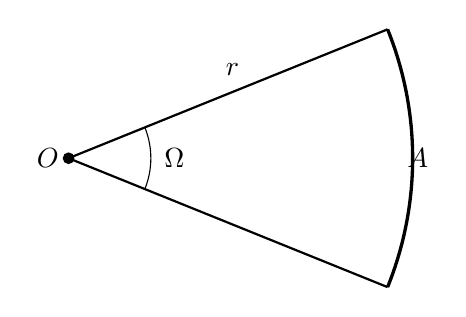
\begin{tikzpicture}[scale=0.95,>=stealth]
  \coordinate (O) at (0,0);
  \draw[thick] (O) -- (22:4.6);
  \draw[thick] (O) -- (-22:4.6);
  \draw[very thick] (22:4.6) arc[start angle=22,end angle=-22,radius=4.6];
  \draw[fill] (O) circle (2pt);
  \node[left] at (O) {$O$};
  \node[above left] at (22:2.6) {$r$};
  \node[right] at (4.4,0) {$A$};
  \draw[thin] (22:1.1) arc[start angle=22,end angle=-22,radius=1.1];
  \node[right] at (1.15,0) {$\Omega$};
\end{tikzpicture}
\end{center}

$\Omega$ যে $r$-এর উপর নির্ভর করে না, সেটি এখন আর ধরে নেওয়ার দরকার নেই; আগের
অনুচ্ছেদের স্কেলিং সূত্রটিই তা বলে দেয়। $r$ দ্বিগুণ করলে একই রশ্মিগুচ্ছ যে টুকরো
কাটে সেটি আগের টুকরোরই সদৃশ, কেবল সব দৈর্ঘ্য দ্বিগুণ; তাই তার ক্ষেত্রফল চার গুণ
হয়। ভাগফল $A/r^{2}$-এ চার গুণ আর চার গুণ কাটাকাটি যায়।

\begin{idea}[পূর্ণ solid angle]
গোলকের সম্পূর্ণ পৃষ্ঠ নিলে $A = 4\pi r^{2}$, সুতরাং একটি বিন্দুর চারপাশে মোট
solid angle
\[
  \Omega_{\mathrm{tot}} = \frac{4\pi r^{2}}{r^{2}} = 4\pi \ \mathrm{sr} .
\]
এটি সমতলে $2\pi$ radian-এর ঠিক ত্রিমাত্রিক প্রতিরূপ।
\end{idea}

\begin{example}
নিচের ক্ষেত্রে solid angle নির্ণয় করো।
\begin{enumerate}
  \item একটি অর্ধগোলক, অর্থাৎ কেন্দ্র থেকে দেখা একটি সমতলের এক পাশের পুরোটা।
  \item ঘরের একটি কোণ, অর্থাৎ তিনটি পরস্পর লম্ব দেয়াল ঘেরা অংশ।
\end{enumerate}
\end{example}

\begin{solbox}
\begin{enumerate}
  \item অর্ধগোলকের পৃষ্ঠ $2\pi r^{2}$, তাই $\Omega = 2\pi$ sr। অর্থাৎ খোলা মাঠে
        দাঁড়িয়ে আকাশের দিকে তাকালে যে পুরো আকাশ দেখা যায়, তার solid angle
        $2\pi$ sr।
  \item তিনটি পরস্পর লম্ব সমতল স্থানকে আটটি সমান অংশে ভাগ করে (প্রতিটি
        স্থানাঙ্কের চিহ্ন ধনাত্মক না ঋণাত্মক, তার আটটি সমন্বয়)। সুতরাং
        \[
          \Omega = \frac{4\pi}{8} = \frac{\pi}{2} \ \mathrm{sr} \approx 1.571 \ \mathrm{sr}.
        \]
\end{enumerate}
\end{solbox}

\begin{example}
চাঁদের ব্যাসার্ধ প্রায় $1.74 \times 10^{6}$ মিটার এবং পৃথিবী থেকে তার দূরত্ব
প্রায় $3.84 \times 10^{8}$ মিটার। পৃথিবী থেকে দেখলে চাঁদ কত solid angle জুড়ে
আছে?
\end{example}

\begin{solbox}
চাঁদ আমাদের কাছে একটি চাকতির মতো দেখায়, যার ক্ষেত্রফল $\pi R^{2}$ যেখানে
$R = 1.74 \times 10^{6}$ মিটার। বস্তুটি যেহেতু দূরত্বের তুলনায় খুব ছোট, ওই সমতল
চাকতির ক্ষেত্রফলকেই গোলকপৃষ্ঠের টুকরোর ক্ষেত্রফল ধরে নেওয়া যায়; এটি একটি
আসন্নীকরণ, তবে এখানে অত্যন্ত ভালো। সুতরাং
\[
  \Omega \approx \frac{\pi R^{2}}{d^{2}}
  = \frac{\pi \left( 1.74 \times 10^{6} \right)^{2}}
         {\left( 3.84 \times 10^{8} \right)^{2}}
  \approx 6.5 \times 10^{-5} \ \mathrm{sr} .
\]
পুরো আকাশের তুলনায় এটি
$\dfrac{6.5 \times 10^{-5}}{4\pi} \approx 5 \times 10^{-6}$ অংশ, অর্থাৎ প্রায়
দুই লক্ষ ভাগের এক ভাগ। এত বড় দেখানো চাঁদ আসলে আকাশের কত সামান্য অংশ জুড়ে আছে,
সংখ্যাটি না কষলে বিশ্বাস করা কঠিন।
\end{solbox}

\begin{remark}
কেন এই ধারণাটা এত গুরুত্বপূর্ণ, তার আভাস দিয়ে রাখি। একটি বিন্দু উৎস থেকে সব
দিকে সমানভাবে কিছু ছড়িয়ে পড়ছে ভাবো: আলো, তাপ, কিংবা বৈদ্যুতিক ক্ষেত্ররেখা।
মোট যা বেরোয় তা $4\pi$ sr-এ ভাগ হয়ে যায়, তাই কোনো নির্দিষ্ট দিকে $\Omega$
solid angle জুড়ে যেটুকু যায় তা মোটের $\Omega/4\pi$ অংশ। এই একটি বাক্য থেকেই
বর্গ-বিপরীত সূত্র (inverse-square law) বেরিয়ে আসে, এবং ২১ নম্বর অধ্যায়ে
Gauss-এর সূত্রও ঠিক এই হিসাবেরই একটি পরিণত রূপ। সেখানে বন্ধ পৃষ্ঠের ভেতরে উৎস
থাকলে সে $4\pi$ sr-এর পুরোটাই জুড়ে থাকে, আর বাইরে থাকলে ভেতরে ঢোকা আর বেরোনো
কাটাকাটি হয়ে শূন্য হয়ে যায়।
\end{remark}

\prob{2} নিচেরগুলো নির্ণয় করো।
\begin{enumerate}
  \item $2$ মিটার $\times$ $2$ মিটার একটি সমতল ফলক $20$ মিটার দূর থেকে লম্বভাবে
        দেখলে তার solid angle কত?
  \item এটি পুরো আকাশের কত ভাগ?
\end{enumerate}

\begin{sol}
\begin{enumerate}
  \item ফলকের ক্ষেত্রফল $4$ বর্গ মিটার এবং দূরত্ব $20$ মিটার। ফলকটি দূরত্বের
        তুলনায় ছোট, তাই
        \[
          \Omega \approx \frac{4}{20^{2}} = \frac{4}{400} = 0.01 \ \mathrm{sr}.
        \]
  \item $\dfrac{0.01}{4\pi} \approx 7.96 \times 10^{-4}$, অর্থাৎ প্রায়
        $0.08$ শতাংশ।
\end{enumerate}
লক্ষ করো, ফলকটি লম্বভাবে না থেকে হেলানো থাকলে তার আপাত ক্ষেত্রফল কমে যেত এবং
solid angle-ও কমত; এখানে লম্ব শর্তটি তাই দরকারি।
\end{sol}

\prob{3} একটি বিন্দু উৎস সব দিকে সমানভাবে $P$ পরিমাণ শক্তি প্রতি সেকেন্ডে ছড়ায়।
\begin{enumerate}
  \item উৎস থেকে দেখা $\Omega$ solid angle জুড়ে থাকা একটি টুকরোর ভেতর দিয়ে
        প্রতি সেকেন্ডে কত শক্তি যায়?
  \item এখান থেকে দেখাও যে $r$ দূরত্বে প্রতি একক ক্ষেত্রফলে প্রতি সেকেন্ডে আসা
        শক্তি $\dfrac{P}{4\pi r^{2}}$।
\end{enumerate}

\begin{sol}
\begin{enumerate}
  \item উৎসের চারপাশে মোট solid angle $4\pi$ sr, আর ছড়ানো সব দিকে সমান। সুতরাং
        $\Omega$ অংশে যায় মোটের $\dfrac{\Omega}{4\pi}$ ভাগ, অর্থাৎ
        \[
          P_{\Omega} = \frac{P\,\Omega}{4\pi} .
        \]
  \item $r$ দূরত্বে $A$ ক্ষেত্রফলের একটি ছোট টুকরো নাও, যা উৎসের দিকে লম্ব।
        তার solid angle $\Omega = A/r^{2}$, তাই তার ভেতর দিয়ে যাওয়া শক্তি
        \[
          P_{\Omega} = \frac{P}{4\pi} \cdot \frac{A}{r^{2}} .
        \]
        প্রতি একক ক্ষেত্রফলে ভাগ করলে $\dfrac{P}{4\pi r^{2}}$।
\end{enumerate}
এটিই বর্গ-বিপরীত সূত্র, এবং খেয়াল করো এতে আলো বা তাপের কোনো ধর্ম ব্যবহার করা
হয়নি; পুরোটাই জ্যামিতি। যা কিছু বিন্দু উৎস থেকে সব দিকে সমানভাবে ছড়ায় এবং পথে
হারায় না, তার জন্যই এটি খাটে।
\end{sol}

\end{document}